\chapter{Theoretical Background}
A complicated point with this kind of subject is the vast field of knowledge that composes it. Indeed, to be able to fully understand the rest of the thesis, it is necessary to have a good knowledge of musical theory rather than an in-depth knowledge of constraint programming. Music theory is very rich and applies differently from one culture to another, while CP is a younger field and easier to popularize broadly. For these reasons, it will be tempted to explain in more depth the sometimes ambiguous musical notions. 

The operation of Gecode and OpenMusic is not necessary for understanding the paper, so they do not have their own sections in this chapter. To learn more about these subjects, there is the documentation of Gecode\parencite{GecodeManual}, OpenMusic\parencite{OpenMusicDoc}, and \textcite{Melothesis}'s thesis which covers the essence of these two tools.

Before moving on to formalization, it is important to recall the fundamentals of music and its notation. The technical theory of constraint programming will be explained right after.
\section{Music Theory}\label{sec:musictheory}
% After the counterpoint has been defined, a glossary of important terms will be given.

\subsection{Concept of Counterpoint}\label{sec:musictheory:counterpoint}
As explained in the introduction, counterpoint (ctp.) is a style predominantly cultivated during the Baroque period. Basically, it involves the simultaneous performance of multiple melodies\parencite{CpSachs}. These melodies exhibit melodic independence while maintaining harmonic interdependence\parencite{CpLaitz}.

\begin{figure}[h]
    \centering
    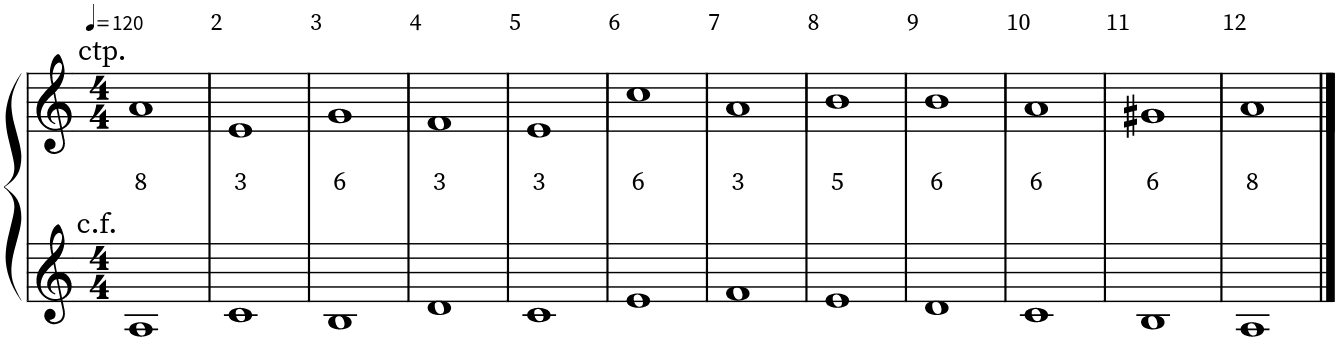
\includegraphics[height=\fhl]{Images/the_first_species.png}
    \caption{Example of a \species{1} ctp. \listen{Listen1SP} \listenyt{https://youtu.be/9yB4OGr4Cgk?t=14}}
\end{figure}

More precisely, each melodic line functions autonomously, possessing its own distinct melodic character, rhythm, and contour. These individual voices are carefully crafted to interact with one another harmonically. While the melodic lines intertwine and intersect, they maintain their melodic independence, allowing each voice to be perceived as a distinct entity within the overall musical composition.

A key element in the construction of counterpoint is the use of a \cfcomma which serves as a foundational melodic line or a "given song." It establishes the melodic and harmonic framework within which the additional voices are developed. Composers use the \cf as a point of departure, building intricate melodic structures around it while adhering to specific rules and guidelines governing melodic and harmonic interactions.

In \citeyear{IMSLPlatin}, \textcite{IMSLPlatin}, a renowned music theorist of the Baroque era, outlined a systematic approach to counterpoint in his influential work, \citetitle{IMSLPlatin}. He categorized counterpoint into five distinct species, each with its own set of rules and characteristics. These species are mainly recognizable by their rhythms. They are built iteratively on top of each other, so that the rules of the first species apply in part in the second species, up to the fifth one.

\begin{itemize}[wide]
    \item First Species: Each note of the added voice corresponds to a single note of the \cfdot The goal is to maintain a strict one-to-one relationship between the voices, ensuring that no dissonances occur.
    \item Second Species: It involves adding two notes in the counterpoint voice for each note of the \cfdot The main added rule is that of allowing dissonant harmonies.
    \item Third Species: Four notes are played in the counterpoint voice against each note of the \cfdot This species introduces more movement and possibilities in the way the melody is handled.
    \item Fourth Species: Mainly composed of syncopations, it focuses on rhythmic displacement and anticipation. The counterpoint voice introduces syncopated rhythms by placing notes on weak beats.
    \item Fifth Species: Also known as the florid counterpoint, it combines elements of the previous four species. It allows for greater freedom in the use of note durations, rhythmic patterns, and melodic embellishments. This species showcases the composer's skill in crafting intricate and ornate melodic lines while maintaining the fundamental principles of counterpoint.
\end{itemize}

\begin{figure}[h]
    \centering
    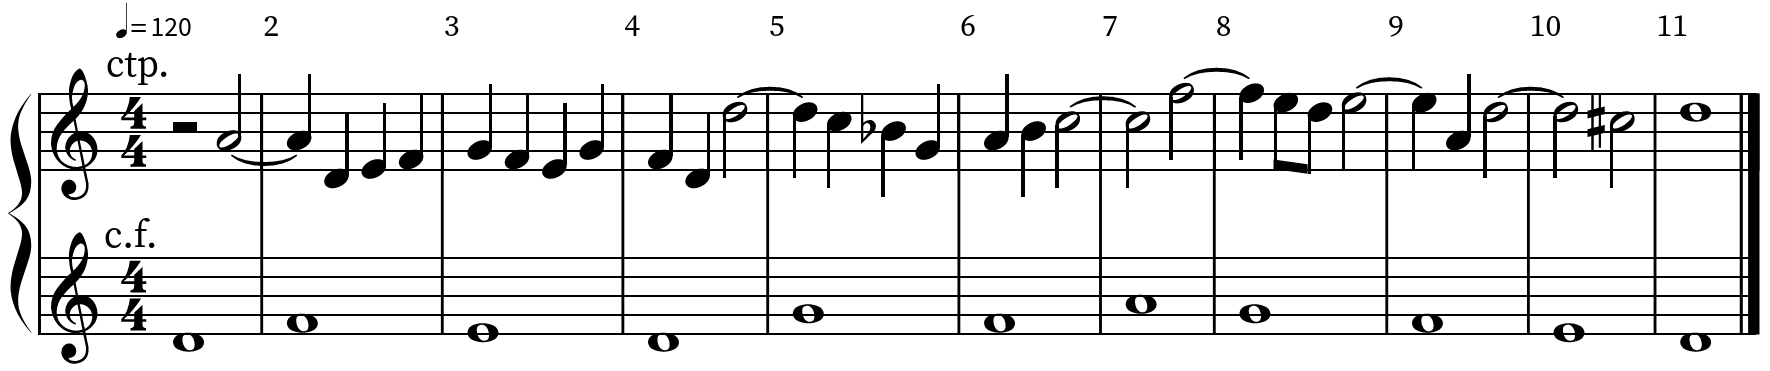
\includegraphics[height=\fhs]{Images/fux_5spA.png}
    \caption{Example of a \species{5} ctp. \listen{Listen5SP} \listenyt{https://youtu.be/9yB4OGr4Cgk?t=231}}
\end{figure}

Don't worry, more examples will be shown in due course.

\subsection{Equivalent American vs British English Terms}
Depending on the reader, terms used in music may vary between America, England, and translations. Here is a summary of the equivalent terms depending on the language:
\begin{multicols}{2}
    \begin{itemize}
        \item Measure $\equiv$ Bar
        \item Whole step $\equiv$ Tone
        \item Half step $\equiv$ Semitone
        \item Whole note $\equiv$ Semibreve
        \item Half note $\equiv$ Minim
        \item Quarter note $\equiv$ Crotchet
        \item Eighth note $\equiv$ Quaver
        \item Sixteenth note $\equiv$ Semi-quaver
    \end{itemize}
\end{multicols}

\subsection{Music Concepts}\label{sec:musictheory:terms}
The following definitions are mainly there to help if the reader does not fully understand the nuances between certain terms in the next chapters. The definitions are sorted so that the first are global and the last are on more specific points.

\paragraph{Staff}
A staff refers to the set of horizontal lines and spaces upon which musical notes and symbols are written on scores. The staff typically consists of five lines and four spaces, with each line and space representing a specific pitch (see figure \ref{fig:theorystaff}).
\begin{figure}[h]
    \centering
    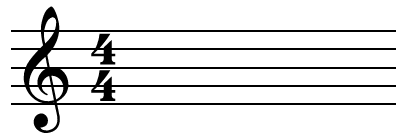
\includegraphics[height=0.5in]{Images/staff.png}
    \caption{Staff with a treble clef (\textit{clef de Sol}), an empty key signature and a 4/4 time signature.}
    \label{fig:theorystaff}
\end{figure}

\paragraph{Note}
On sheet music, a note is a symbol used to represent a specific pitch and duration of a sound. Notes are written on staff and can be represented by a variety of symbols. Generally speaking, a note refers to a certain frequency played at a certain time.

\paragraph{Beat} A beat is the underlying pulse that organizes the passage of time within a musical composition. It serves as a fundamental unit of measurement, establishing the division of time into equal segments. The beat provides a sense of stability and acts as the rhythmic foundation upon which melodies, harmonies, and other musical elements are built.

\paragraph{Measure}
A measure is a section of music that is delimited by vertical bar lines in sheet music. With a common 4/4 time signature, a measure is made up of four beats.

\paragraph{Pitch}
Pitch refers to the highness or lowness of a sound. Pitch is determined by the frequency of the sound wave and is measured in hertz (Hz). Higher pitched sounds have a higher frequency than lower pitched sounds.

\paragraph{MIDI} \textit{Musical Instrument Digital Interface} is a standard protocol for communication between musical instruments and computers. What is commonly called "MIDI values" refers to the different possible MIDI notes ranging from 0 ($C_{-1} \equiv 8.175799\ Hz$) to 127 ($G_{9} \equiv 12543.85\ Hz$)\parencite{MIDIwiki}. The notes of an 88-key piano are limited to $A_0$ to $C_8$. The list of MIDI values can be found in table \ref{tab:midivalues}.

\paragraph{Semitone}
A semitone, also known as a half step, is the smallest interval (the distance between two notes) in Western music. It represents the distance between two adjacent notes on a keyboard or guitar.

\paragraph{Step} A step is a melodic interval of one semitone (minor second) or one tone (major second)\parencite{Step} between two consecutive notes of a musical scale\parencite{Stepswiki}. Melodies that move by steps are \emph{stepwise}.

\paragraph{Types of notes}
Within a common 4/4 time signature (see figure \ref{fig:theorytypesofnotes}):
\begin{multicols}{3}
    \begin{itemize}
        \item A \textbf{whole note} represents a long duration of sound and lasts four beats.
        \item A \textbf{half note} represents a medium duration of sound and lasts two beats.
        \item A \textbf{quarter note} represents a short duration of sound and lasts one beat.
    \end{itemize}
\end{multicols}

\begin{figure}[h]
    \centering
    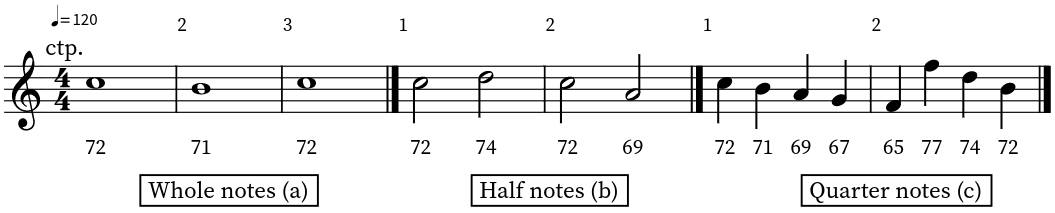
\includegraphics[height=1in]{Images/melodic_intervals_variables.png}
    \caption{The 3 main types of notes used in the counterpoint.}
    \label{fig:theorytypesofnotes}
\end{figure}

\paragraph{Syncopation} The displacement of the main beat of a measure. It creates an off-balance rhythm through the accenting of normally unaccented beats.

\paragraph{Mordent} A mordent is a type of ornament referring to a quick alternation between a note and its upper (upper mordent) or lower neighbor (lower/inverted mordent)\parencite{Mordent}.

\paragraph{Intervals}
In Western tonal music, the intervals making up an octave are separated into 12 semitones. Table \ref{tab:intervalsvalues} shows the MIDI values corresponding to these intervals.
\begin{table}[!h]
    \centering
    \resizebox{\columnwidth}{!}{%
        \begin{tabular}{|c||c|cc|cc|c|c|c|cc|cc|}
            \hline
            Interval                           &
            Unison/Octave                      &
            \multicolumn{2}{c|}{Second}        &
            \multicolumn{2}{c|}{Third}         &
            Fourth                             & Tritone                    & Fifth &
            \multicolumn{2}{c|}{Sixth}         &
            \multicolumn{2}{c|}{Seventh}                                                                           \\ \hline
            Type                               &
            Perfect                            & \multicolumn{1}{c|}{Minor} &
            Major                              & \multicolumn{1}{c|}{Minor} &
            Major                              & Perfect                    &
            $\sharp \nth{4}$ / $\flat \nth{5}$ &
            Perfect                            & \multicolumn{1}{c|}{Minor} &
            Major                              & \multicolumn{1}{c|}{Minor} &
            Major                                                                                                  \\ \hline
            Value                              &
            0                                  & \multicolumn{1}{c|}{1}     &
            2                                  & \multicolumn{1}{c|}{3}     &
            4                                  & 5                          & 6     & 7 & \multicolumn{1}{c|}{8} &
            9                                  & \multicolumn{1}{c|}{10}    &
            11                                                                                                     \\ \hline
        \end{tabular}
    }
    \caption{MIDI values of the intervals over an octave range.}
    \label{tab:intervalsvalues}
\end{table}

\paragraph{Tonic}
The tonic is the first note of a scale and serves as the foundation or the "home" for the other notes in the scale. It is this note that gives the name of the scale.

\paragraph{Scale}
A scale is a series of intervals arranged in ascending or descending order. The most common scales in Western music are the major and minor scales. Each scale has a unique pattern of whole and half steps between the notes.

\paragraph{Key}
A key refers to a specific scale and tonic. For example, a piece of music in the key of C major would use the major scale and have C as the tonic. The key of a piece of music determines the overall tonality and harmony of the piece.

\paragraph{Mode}
A mode is a type of scale that can be seen as a derivation from a parent scale. Basically, they are alternatives to common scales so that the tonic and the other note functions have been shifted. The modes in Western music are the Dorian, Phrygian, Lydian, Mixolydian, Aeolian, and Locrian modes. Like any scale, each mode has a unique pattern of whole and half steps between the notes.

\paragraph{Diatonic}
A diatonic scale is a scale made up of seven different pitches, where each pitch corresponds to a letter in the musical alphabet ($A, B, C, D, E, F, G$). A note is considered diatonic if it belongs to the key range of the piece.

\paragraph{Chromatic}
A chromatic scale is a scale that includes all the notes separated by a semitone. A chromatic scale contains 12 notes in total, including all the notes in a diatonic scale and additional notes between each of the diatonic scale notes. Chromatic notes are often used to add dissonance or tension to a piece of music.

\paragraph{Borrowed note}
A borrowed note is a non-diatonic note borrowed from another key or mode and used temporarily in a piece of music. Borrowed notes can be used to add variety and interest to a melody or harmony. They can also be used to create a sense of tension or dissonance, which can then be resolved back to the original key or mode.

\paragraph{Degree} A degree is the relative position of a note in a scale to the tonic. By default, one degree aside from a note is the closest next note available in the diatonic scale. A degree can be expressed for both melody and harmony (even as chords). The degrees make it possible to understand and convert any tonality through a relative system\parencite{Degree}. By convention, they are written with Roman numerals from I (the tonic) to VII (the sensible). For example, in $C$ major, $C$ (i.e. the tonic) is the I degree while $G$ (i.e. the dominant, the fifth) is the V degree. Transposed to $F$ major, this would give $F$ the I degree and $C$ the V degree. Also, melodies that progress by joint degrees are equivalent to stepwise melodies.

\paragraph{Thesis} Aka downbeat. With a common 4/4 time signature, the thesis is the first beat of any measure.

\paragraph{Arsis} Aka upbeat. With a common 4/4 time signature, the arsis is the third beat of any measure.

\paragraph{Skip} The melodic interval which, unlike the step, is greater than one tone. The term is rather used to refer to the third melodic interval because it is equivalent to \textit{skip} a key on a piano but no convention exists. "Leap" can therefore also be used for the same purpose.

\paragraph{Leap} The melodic interval which, unlike the step, is greater than one tone. The term is rather used to refer to melodic intervals larger than a third in contrast with the term "skip". Although, no convention exists so "skip" can also be used for the same purpose.

\paragraph{Diminution} An intermediate note that exists between two notes separated by a skip of a third. In other words, a note that fills the space in third skip. This intermediate note is not necessarily below the previous one. Actually, the term refers to the division of a note into several shorter ones (i.e. "passage notes")\parencite{Diminution}.
\section{Constraint Programming Prerequisites}
This thesis is more focused on mathematical formalization than on the extensive use of constraint programming. Indeed, as will be explained later, optimization is not a point that was particularly highlighted during this work. The limits of Gecode were not reached within the framework of this work. There was thus no need to investigate in that specific direction. Despite this, it is still important to understand what constraint programming is. 

\subsection{Constraint Programming Concept}
Constraint programming is an approach to solve complex combinatorial problems by specifying them as logical relations, called constraints\parencite{CPbook}. This kind of problem is called \textit{constraint satisfaction problem} or CSP. It is solved by using a combination of inference and search. CP is a powerful paradigm in the field of computer science that addresses complex decision-making and optimization problems.

Problems are represented as a set of variables, each with a domain of possible values, and constraints that define the allowable combinations of values for these variables. Constraints capture logical relationships between variables, reflecting the problem's requirements.

The solver part has to find a solution that satisfies all the given constraints by determining the values for the variables that do not violate previously posted constraints. In practice, CP engines employ constraint propagation techniques to enforce the constraints and reduce the search space by propagating the effects of variable assignments.

\subsection{Branching}
Branching refers to the selection of variables and their values during the exploration of the solution space. It involves selecting a variable and dividing its domain into smaller subsets or branches, each representing a possible assignment.

When solving a CSP with Gecode, there are two fundamental search strategies employed: depth-first search and branch-and-bound. These strategies are guided by variable selection heuristics and value selection heuristics. Without going into details, depth-first search assigns values to variables regarding the heuristics and then backtracks when constraints cannot be satisfied. The branch-and-bound strategy extends depth-first search by incorporating an additional mechanism to post a new constraint specified in advance\footnote{With the current version of GiL, it has never been possible to make branch-and-bound work from Lisp. Several attempts were tested but all failed.}.

The choice of variable for branching is guided by variable selection heuristics, which determine the order in which variables are considered during the search process. These heuristics aim to select the most promising variable at each step, leading to faster convergence. Common variable selection heuristics include selecting the variable with the fewest remaining values in its domain (minimum domain size) or selecting the variable involved in the most constraints (maximum degree). Value selection heuristics determine the order in which values are assigned to variables. These heuristics aim to prioritize values that are more likely to lead to a successful solution.

\subsection{Advantages}
To summarize the benefits that lead to the use of CP, it can be said that it mainly stands out for its expressiveness, transparency, flexibility, and efficiency. CP allows problem solvers to express problems in a natural manner, enabling direct communication of knowledge and requirements. It provides transparency in the problem-solving process, making search algorithms and strategies explicit and understandable. CP supports flexible problem modeling, allowing the incorporation of additional constraints, objectives, and problem-specific knowledge. It can efficiently explores the solution space using constraint propagation and search techniques, reducing the search space and quickly discarding infeasible solutions. These advantages make CP valuable for addressing a wide range of real-world decision-making and optimization problems.